%!TEX root = edance.tex
%%%%%%%%%%%%%%%%
%   CHAPTER 8  %
%%%%%%%%%%%%%%%%
\chapter{MOSFET Device Physics}
\label{ch:ch08_mos}
\graphicspath{{./figs_mos/}}
%%%%%%%%%%%%%%%%%%%%%%%%%%%%%%%%%%%%%%%%%%%%%%%%%%%%%%%%%%%%%%%%%%%%%%%%%%%%%%%%%%%%%%%%
%%%%%%%%%%%%%%%%%%%%%%%%%%%%%%%%%%%%%%%%%%%%%%%%%%%%%%%%%%%%%%%%%%%%%%%%%%%%%%%%%%%%%%%%
%                                   SECTION 8.1                                        %
%%%%%%%%%%%%%%%%%%%%%%%%%%%%%%%%%%%%%%%%%%%%%%%%%%%%%%%%%%%%%%%%%%%%%%%%%%%%%%%%%%%%%%%%
%%%%%%%%%%%%%%%%%%%%%%%%%%%%%%%%%%%%%%%%%%%%%%%%%%%%%%%%%%%%%%%%%%%%%%%%%%%%%%%%%%%%%%%%
\section{Chapter Preview}
A MOSFET, or MOS Field Effect Transistor, is a device constructed from a MOS capacitor by adding two extra diffusion regions, shown in Fig.~\ref{fig:mosfet_layout}.  We begin the chapter by discussing the structure of the MOSFET, discussing the different flavors of MOS technology, including NMOS and PMOS devices, and CMOS technology.  The difference between these devices will be discussed in detail.  Next we examine the current-voltage characteristics of a MOSFET, known as the $I$-$V$ curves.  Similar to a resistor, we can plot current versus voltage for a MOSFET, but given that the device has three terminals, we must plot families of curves.  Once we have an phenomenological understanding of the MOSFET, we derive analytical equations for an ideal "long channel" device.  This will lead us into understanding some important concepts in the MOSFET, such as the current saturation mechanism.  Finally, we end the chapter by discussing the PMOS device, which is completely complementary to the NMOS device.
%%%%%%%%%%%%%%%%%%%%%%%%%%%%%%%%%%%%%%%%%%%%%%%%%%%%%%%%%%%%%%%%%%%%%%%%%%%%%%%%%%%%%%%%
%%%%%%%%%%%%%%%%%%%%%%%%%%%%%%%%%%%%%%%%%%%%%%%%%%%%%%%%%%%%%%%%%%%%%%%%%%%%%%%%%%%%%%%%
%                                   SECTION 8.2                                        %
%%%%%%%%%%%%%%%%%%%%%%%%%%%%%%%%%%%%%%%%%%%%%%%%%%%%%%%%%%%%%%%%%%%%%%%%%%%%%%%%%%%%%%%%
%%%%%%%%%%%%%%%%%%%%%%%%%%%%%%%%%%%%%%%%%%%%%%%%%%%%%%%%%%%%%%%%%%%%%%%%%%%%%%%%%%%%%%%%
\section{MOSFET Device Layout and Cross Section}
%%%%%%%%%%%%%%%%%%%%%%%%%%%%%%%%%%%%%%%%%%%%
%             SUBSECTION 8.2.1             %
%%%%%%%%%%%%%%%%%%%%%%%%%%%%%%%%%%%%%%%%%%%%
\subsection{MOSFET Top View and Layout}
%%%%%%%%%%%%%%%%%%%%%%%%%%%%%%%%%%%%%%%%%%%%
%                 FIGURE                   %
%%%%%%%%%%%%%%%%%%%%%%%%%%%%%%%%%%%%%%%%%%%%
\begin{figure}[tb]
\centering
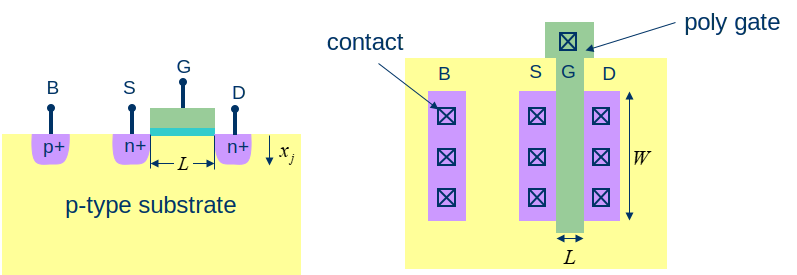
\includegraphics[width=.95\columnwidth]{mosfet_layout}
\caption{Cross section (left) and top-level layout of a MOSFET device (right).  In general, the device has four terminals, lableled (G) gate, (B) body, (S) source, and (D) drain.  The layout parameters include the width $W$ and length $L$.}
\label{fig:mosfet_layout}
\end{figure}
%%%%%%%%%%%%%%%%%%%%%%%%%%%%%%%%%%%%%%%%%%%%
The cross-section and top view of a MOSFET are shown in Fig.~\ref{fig:mosfet_layout}.  A MOS transistor is four terminal device that conducts current between two of its terminals under the control of the third terminal, the "gate" (G).  In a MOSFET, the terminals that carry current are known as the "drain" (D) and "source" (S), in analogy with liquid flow.  The "source" supplies electrons, and they flow from the source to the drain.  Since electrons carry negative charge, the current from is from the drain to the source, which is confusing but standard convention.  The fourth terminal is the "body" (B), which establishes a potential reference for the gate terminal.  Often the body and source are shorted together, and this leads to a "source referenced" notion of the gate voltage.  In general, it's the gate-to-body voltage that determines the operating point of the MOS-C and therefore the MOSFET.
%%%%%%%%%%%%%%%%%%%%%%%%%%%%%%%%%%%%%%%%%%%%
From the top view of the MOSFET shown in Fig.~\ref{fig:mosfet_layout}, it's important to note that the dimensions $L$ and $W$ are layout dependent and can be varied by the circuit designer.  These parameters control the size of the channel that forms from the source to drain to conduct current when the device is biased in inversion.  The parameter $W$ is the device width, and the larger the width, the more current the transistor can conduct.  The device dimension $L$ is the channel length, and  the shorter the channel, the more conductive the channel.  The smallest possible dimension $L_{min}$ is a technology-dependent parameter as manufacturers strive to improve the performance of the device by providing means of fabricating smaller and smaller devices.  Today's transistors are fabricated with channel lengths as small as 7nm but not all applications need such a small device.  Generally speaking, smaller channel length leads to a smaller required $W$ to get the same current, and therefore an overall smaller device, which favors high density logic where millions to billions of transistors are fabricated on a single chip.  In analog circuit applications, requirements are different and much larger devices may be employed.  Today, devices as large as $1\mathrm{\mu m}$ are used in power and automotive applications and short channel devices down to 22nm are routinely used for RF (radio frequency) applications.  
%%%%%%%%%%%%%%%%%%%%%%%%%%%%%%%%%%%%%%%%%%%%
%                 FIGURE                   %
%%%%%%%%%%%%%%%%%%%%%%%%%%%%%%%%%%%%%%%%%%%%
\begin{figure}[tb]
\centering
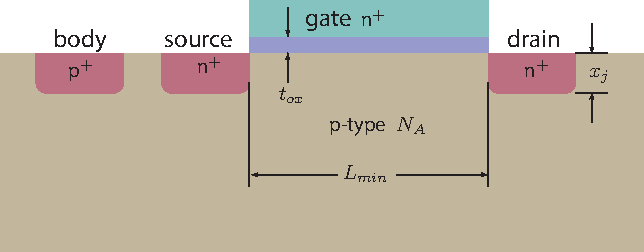
\includegraphics[width=.75\columnwidth]{mos_tech}
\caption{Cross section of a MOSFET device. Important technology parameters include the minimum channel length $L_{min}$, the body doping ($N_A$), the oxide thickness ($t_{ox}$), and the junction depth $x_j$.}
\label{fig:mos_tech}
\end{figure}
%%%%%%%%%%%%%%%%%%%%%%%%%%%%%%%%%%%%%%%%%%%%
Another thing worth mentioning is that MOSFET devices are "planar".  In the figure, note that $x_j$ is the junction depth, and the channel will form at the surface of the device.  While the metal stack-up (see Fig.~\ref{fig:cmos_photo}) may be three dimensional, the actual transistors all reside in a thin layer at the surface of the body.  The circuit designers usually only control the 2D layout of the device, as the third dimension (junction depth for instance) is set by technologist to achieve the best performance.  The most important technology parameters, highlighted in Fig.~\ref{fig:mos_tech}, include the minimum channel length $L_{min}$, oxide thickness $t_{ox}$, the device body doping $N_A$, and the junction depth $x_j$.
%%%%%%%%%%%%%%%%%%%%%%%%%%%%%%%%%%%%%%%%%%%%
%                 FIGURE                   %
%%%%%%%%%%%%%%%%%%%%%%%%%%%%%%%%%%%%%%%%%%%%
\begin{figure}[tb]
\centering
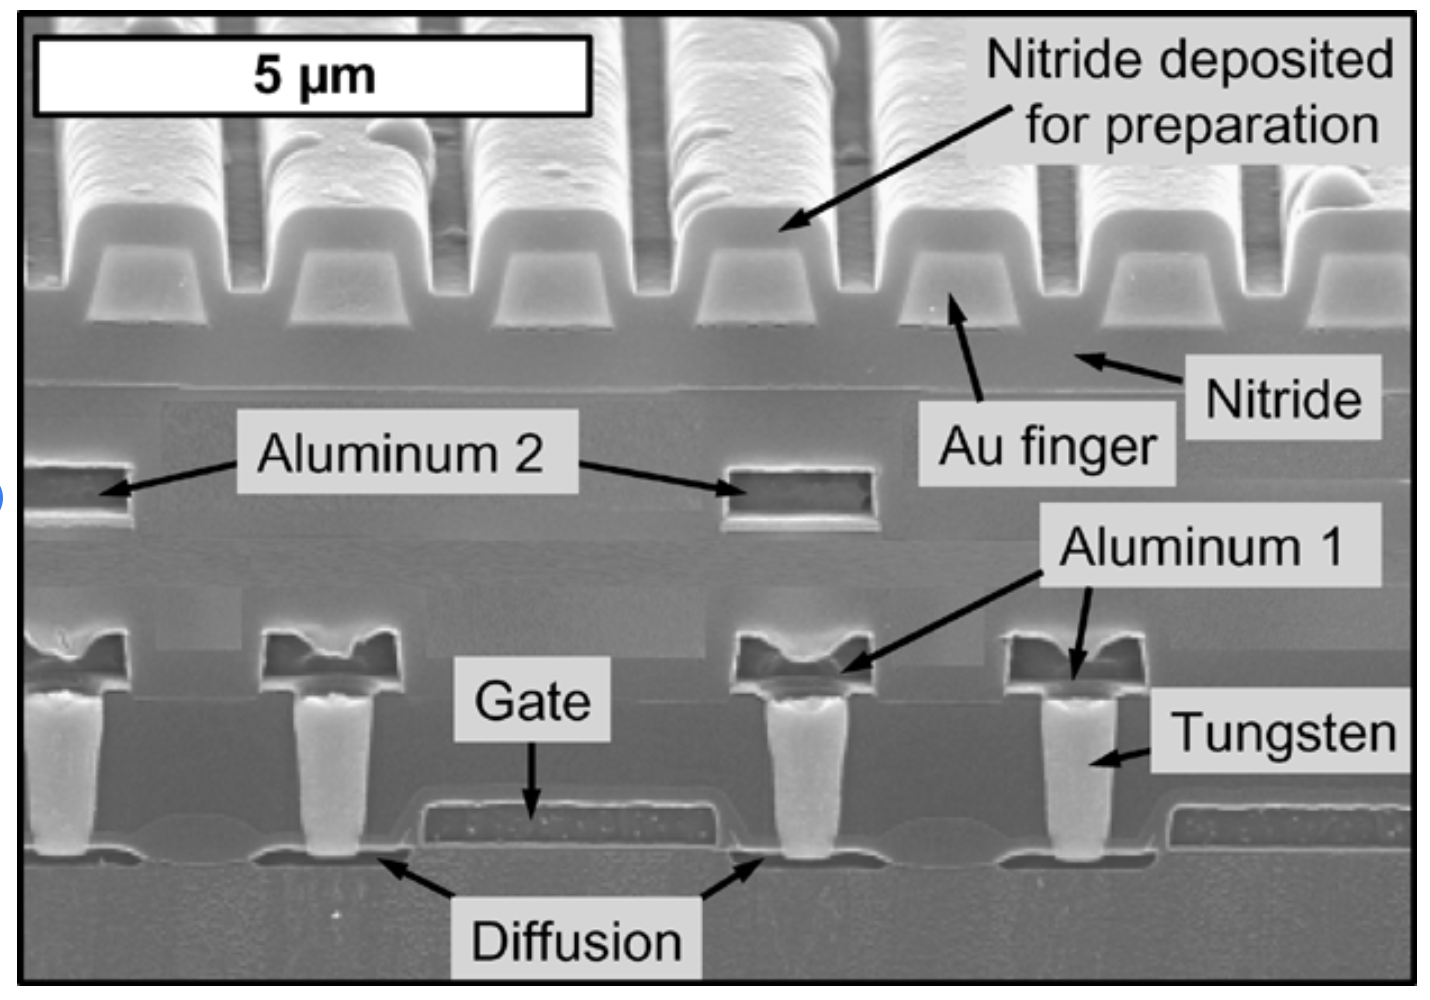
\includegraphics[width=.65\columnwidth]{cmos_xsection_photo.png}
\caption{SEM cross-section photo of a CMOS chip. {\small(Used without permission from M. Schienle et al., "A fully electronic DNA sensor with 128 positions and in-pixel A/D conversion," in \emph{IEEE Journal of Solid-State Circuits}, vol. 39, no. 12, pp. 2438-2445, Dec. 2004.)}}
\label{fig:cmos_photo}
\end{figure}
%%%%%%%%%%%%%%%%%%%%%%%%%%%%%%%%%%%%%%%%%%%%
%             SUBSECTION 8.2.2             %
%%%%%%%%%%%%%%%%%%%%%%%%%%%%%%%%%%%%%%%%%%%%
\subsection{MOSFET Overview}
With a solid understanding of a MOS capacitor, we now introduce the MOS transistor, or MOSFET.  Note that to make a MOSFET, we start with a MOS capacitor and add two diffusion regions adjacent to the gate, shown in Fig.~\ref{fig:mos_tech}.  Note the doping of these regions is opposite to the body of the device.  For a $P$-type substrate, we dope the drain and source $N$-type and make contact with the source and drain terminals.  These junctions form reverse biased (under proper biasing conditions) diodes between the source/drain and the body of the transistor.  Unless we "turn on" the device, no current can flow between the source and drain because of the presence of two back-to-back diodes.  When a sufficiently large gate voltage is applied, the surface of the MOS-C is inverted, creating a channel between the source and drain, allowing current to flow (see Fig.~\ref{fig:mos_current}).    
%%%%%%%%%%%%%%%%%%%%%%%%%%%%%%%%%%%%%%%%%%%%
It's important to note that the MOSFET is a four terminal device, but in most situations the body terminal is connected to a fixed DC voltage, or shorted to the source.  The reason for this will become clear later but for now you can assume that unless otherwise noted, the body of the device is connected to ground for NMOS devices and connected to the supply (or highest potential) for a PMOS device.  These connections ensure that under normal operating conditions, when the source and drain voltages swing between ground and supply, the diodes remain reverse biased.
%%%%%%%%%%%%%%%%%%%%%%%%%%%%%%%%%%%%%%%%%%%%
%                 FIGURE                   %
%%%%%%%%%%%%%%%%%%%%%%%%%%%%%%%%%%%%%%%%%%%%
\begin{figure}[tb]
\centering
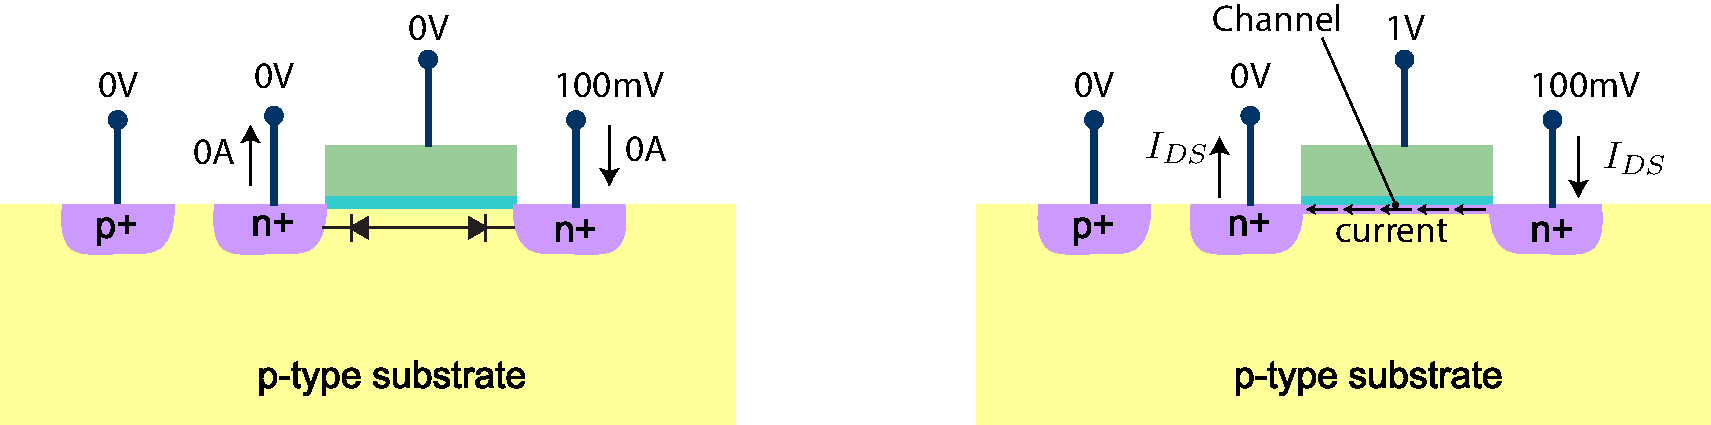
\includegraphics[width=\columnwidth]{mostfetxsect_current} 
\caption{Cross section of an NMOS device with (a) a zero gate voltage is "off" and cannot conduct current whereas, and (b) a sufficiently positive gate voltage is applied to turn "on" the device, allowing electrons to flow from the source to the drain.}
\label{fig:mos_current}
\end{figure}
%%%%%%%%%%%%%%%%%%%%%%%%%%%%%%%%%%%%%%%%%%%%
%             SUBSECTION 8.2.3             %
%%%%%%%%%%%%%%%%%%%%%%%%%%%%%%%%%%%%%%%%%%%%
\subsection{MOSFET Flavors:  PMOS and NMOS}
MOSFETs are also known by other names, namely the IGFET, or Insulated Gate Field-Effect Transistors.  This name is not really in common use, and MOSFET is much more common.  FETs are a general class of devices that include other devices such as Junction FETS (J-FET or JFET) and Metal-Semiconductor FETs, or MESFETs.  We will focus on MOSFETs in this book, although the behavior of MOSFETs, JFETs, and MESFETs are all very similar from the high level perspective of design.  In fact, we'll show in the next chapter that by employing small-signal models, all devices essentially look the same.
%%%%%%%%%%%%%%%%%%%%%%%%%%%%%%%%%%%%%%%%%%%%
%                 FIGURE                   %
%%%%%%%%%%%%%%%%%%%%%%%%%%%%%%%%%%%%%%%%%%%%
\begin{figure}[tb]
\centering
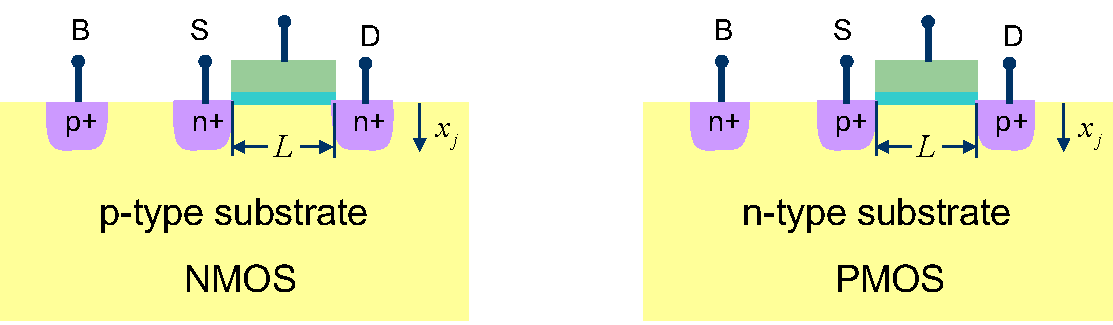
\includegraphics[width=.75\columnwidth]{pmos_xsect}
\caption{Cross section of a PMOS device is very similar to an NMOS device, except it's realized by using an $N$-type body doping and p$^+$ doping diffusion regions to define the source and drain.} \label{fig:pmos_xsect}
\end{figure}
%%%%%%%%%%%%%%%%%%%%%%%%%%%%%%%%%%%%%%%%%%%%
For a given technology, it may be possible to fabricate two complementary devices, shown in Fig.~\ref{fig:pmos_xsect}.  For example, in this chapter we'll see that we can fabricate a MOSFET on a $P$-type body (often the substrate), resulting in an NMOS or NFET device, or on an $N$-type body, resulting in a PMOS or PFET device.  These devices are complementary in the sense that the currents and voltages are all in essence the negative of each other.  We already saw this with a MOS-C, where for an $N$-type device a sufficiently positive gate voltage results in inversion, whereas for a $P$-type MOS-C, a negative gate-to-body voltage is needed. The same is true of MOSFET devices.
%%%%%%%%%%%%%%%%%%%%%%%%%%%%%%%%%%%%%%%%%%%%
%             SUBSECTION 8.2.4             %
%%%%%%%%%%%%%%%%%%%%%%%%%%%%%%%%%%%%%%%%%%%%
\subsection{CMOS Technology}
Finally we should discuss the term "CMOS", which stands for "Complementary MOS," or a technology capability to fabricate both NMOS and PMOS devices.  CMOS technology is now universal for silicon-based technology.  As shown in Fig.~\ref{fig:cmos_xsect}, both devices are fabricated on the same substrate by creating wells (oppositely doped to the body) to house devices.  With a $P$-type substrate shown, the NMOS devices can be fabricated directly in the body, and the PMOS devices are fabricated in so-called n-well regions.  These well regions are counter-doped to make them $N$-type, and then $P$-type source/drain junctions are added to make the PMOS device.  The wells need to be biased such that at all times the well-to-body diode is reverse biased.  The well bias is established through the body connection.
%%%%%%%%%%%%%%%%%%%%%%%%%%%%%%%%%%%%%%%%%%%%
%                 FIGURE                   %
%%%%%%%%%%%%%%%%%%%%%%%%%%%%%%%%%%%%%%%%%%%%
\begin{figure}[tb]
\centering
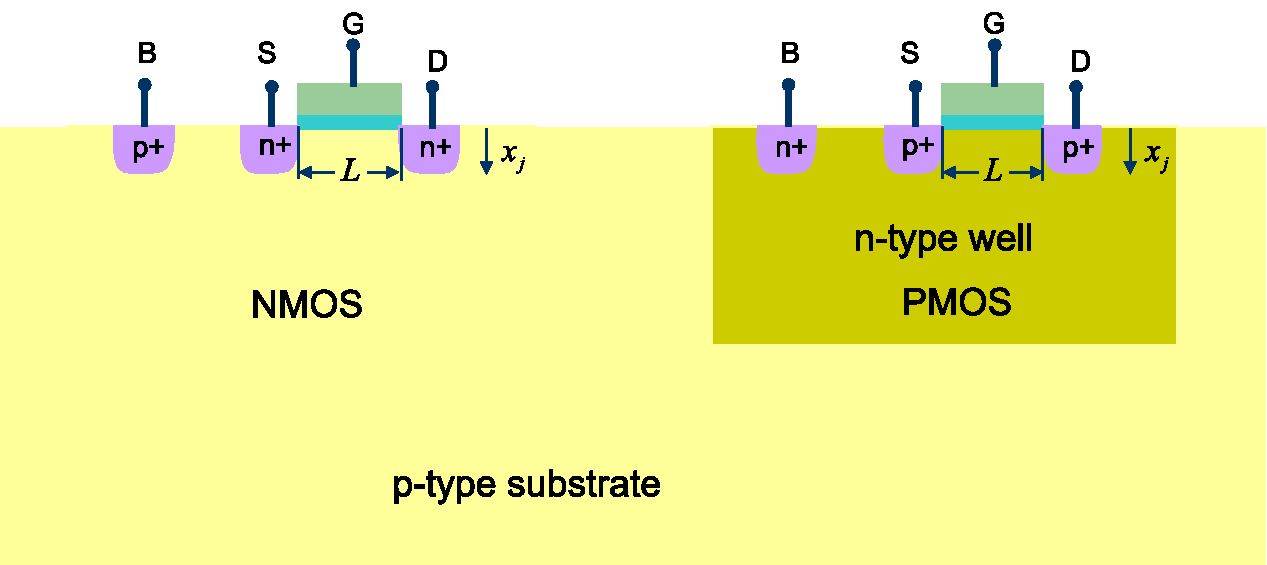
\includegraphics[width=.85\columnwidth]{cmos_xsect}
\caption{CMOS technology allows one to build both NMOS and PMOS devices in the same technology side-by-side as shown.  NMOS devices are realized directly using the $P$-type substrate as the body whereas the PMOS device requires a "well", a region counter-doped $N$-type to realize the PMOS body.}
\label{fig:cmos_xsect}
\end{figure}
%%%%%%%%%%%%%%%%%%%%%%%%%%%%%%%%%%%%%%%%%%%%
%             SUBSECTION 8.2.5             %
%%%%%%%%%%%%%%%%%%%%%%%%%%%%%%%%%%%%%%%%%%%%
\subsection{Circuit Symbols}
%%%%%%%%%%%%%%%%%%%%%%%%%%%%%%%%%%%%%%%%%%%%
%                 FIGURE                   %
%%%%%%%%%%%%%%%%%%%%%%%%%%%%%%%%%%%%%%%%%%%%
\begin{figure}[tb]
\centering
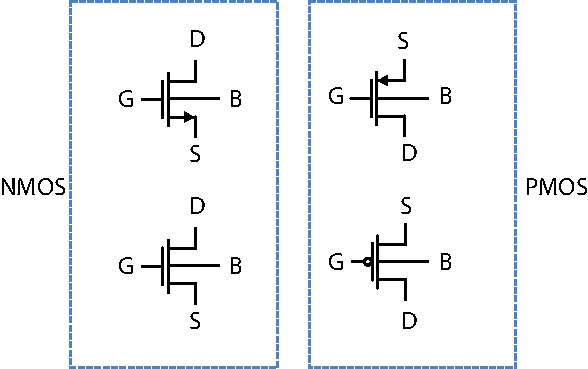
\includegraphics[width=.6\columnwidth]{mos_symbols}
\caption{Schematic symbols for the NMOS and PMOS devices.}
\label{fig:mos_symbols}
\end{figure}
%%%%%%%%%%%%%%%%%%%%%%%%%%%%%%%%%%%%%%%%%%%%
In circuit schematics MOSFET symbols are drawn as shown in Fig.~\ref{fig:mos_symbols}.  The symbols with the arrows are more common in analog circuit applications, and the symbols with the bubble on the gate for PMOS are more favored in digital applications.  The bubble emphasizes that the PMOS device is the logical "NOT" of the NMOS device. In other words, a low voltage is needed to turn on the PMOS device (with respect to the body), whereas for the NMOS device a high voltage (relative to the body) is needed.  The arrows in the symbol denote the typical direction of current flow (not electron flow).  Since the source and drain are often physically the same, the actual drain/source may be swapped.  The source and drain are really only meaningful when the bias voltages are specified. For an NMOS device, to get current to flow from the drain-to-source, the drain should be at a higher potential than the source.  The opposite is true for the PMOS device.
%%%%%%%%%%%%%%%%%%%%%%%%%%%%%%%%%%%%%%%%%%%%
The body terminal is sometimes omitted from the schematic for clarify.  In this situations its implicit that the body of all NMOS devices is tied to ground, or the lowest potential, and the body of all PMOS devices is connected to the supply, or highest potential.
%%%%%%%%%%%%%%%%%%%%%%%%%%%%%%%%%%%%%%%%%%%%%%%%%%%%%%%%%%%%%%%%%%%%%%%%%%%%%%%%%%%%%%%%
%%%%%%%%%%%%%%%%%%%%%%%%%%%%%%%%%%%%%%%%%%%%%%%%%%%%%%%%%%%%%%%%%%%%%%%%%%%%%%%%%%%%%%%%
%                                   SECTION 8.3                                        %
%%%%%%%%%%%%%%%%%%%%%%%%%%%%%%%%%%%%%%%%%%%%%%%%%%%%%%%%%%%%%%%%%%%%%%%%%%%%%%%%%%%%%%%%
%%%%%%%%%%%%%%%%%%%%%%%%%%%%%%%%%%%%%%%%%%%%%%%%%%%%%%%%%%%%%%%%%%%%%%%%%%%%%%%%%%%%%%%%
\section{NMOSFET Large Signal Models and Regions of Operation}
We begin by looking at the MOSFET as MOS-C and note the importance of the gate-to-body voltage.  Next we look at the device as a black box in order to understand the drain-source current-voltage behavior.  Later we'll use this insight to derive the analytical equations.
%%%%%%%%%%%%%%%%%%%%%%%%%%%%%%%%%%%%%%%%%%%%
%             SUBSECTION 8.3.1             %
%%%%%%%%%%%%%%%%%%%%%%%%%%%%%%%%%%%%%%%%%%%%
\subsection{Cut-off\texorpdfstring{$,\;V_{GS}<V_T$}{}}
%%%%%%%%%%%%%%%%%%%%%%%%%%%%%%%%%%%%%%%%%%%%
%                 FIGURE                   %
%%%%%%%%%%%%%%%%%%%%%%%%%%%%%%%%%%%%%%%%%%%%
\begin{figure}[tb]
\centering
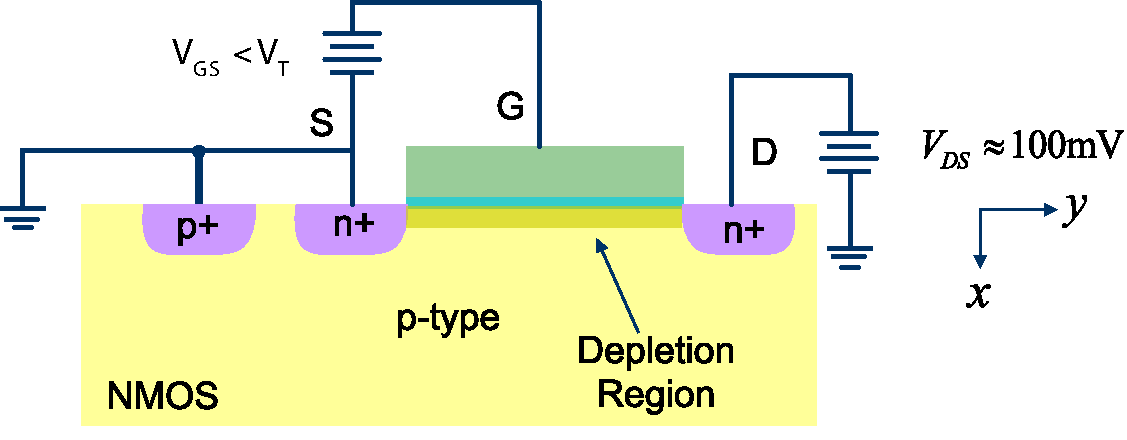
\includegraphics[width=.75\columnwidth]{mos_cutoff}
\caption{The MOS device biased in cut-off, or a gate bias $V_{GS} < V_T$, cannot conduct any current as the source and drain are isolated by two back-to-back diodes and a depletion region.}
\label{fig:mos_cutoff}
\end{figure}
%%%%%%%%%%%%%%%%%%%%%%%%%%%%%%%%%%%%%%%%%%%%
As shown in Fig.~\ref{fig:mos_cutoff}, we can look at the MOSFET as a MOS capacitor with two n$^+$ diffusion regions on each side. When $V_{GB} < V_T$, the device is either in accumulation or in depletion. Since there are no (or very few) inversion charges at the surface, there is no path for current to flow from the source to the drain.  No matter how large we make $V_{DS}$ (up to breakdown limits), current does not flow through two back-to-back diodes that are of opposite polarity.
%%%%%%%%%%%%%%%%%%%%%%%%%%%%%%%%%%%%%%%%%%%%
%             SUBSECTION 8.3.2             %
%%%%%%%%%%%%%%%%%%%%%%%%%%%%%%%%%%%%%%%%%%%%
\subsection{Inversion\texorpdfstring{$,\;V_{GS}>V_T\text{and}V_{DS}>0$}{}}
%%%%%%%%%%%%%%%%%%%%%%%%%%%%%%%%%%%%%%%%%%%%
%                 FIGURE                   %
%%%%%%%%%%%%%%%%%%%%%%%%%%%%%%%%%%%%%%%%%%%%
\begin{figure}[tb]
\centering
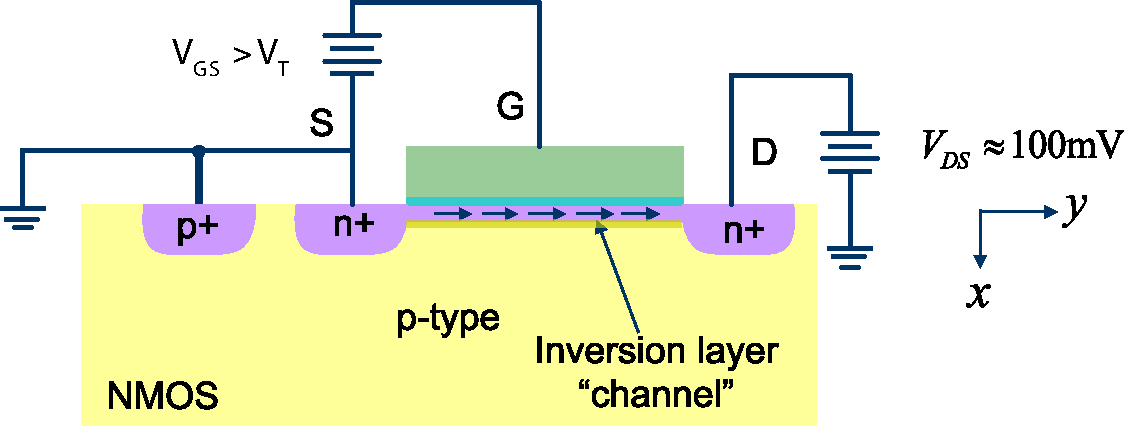
\includegraphics[width=.75\columnwidth]{mos_triode}
\caption{When a sufficiently positive gate voltage is applied, $V_{GS} > V_T$, a channel forms between the drain and source, essentially connecting these regions.  Electrons can be injected into the channel from the source side, and flow to the drain (biased at a higher potential).  Note current flow is in the opposite direction due to electron charge.}
\label{fig:mos_triode}
\end{figure}
%%%%%%%%%%%%%%%%%%%%%%%%%%%%%%%%%%%%%%%%%%%%
On the other hand, if the gate is biased above threshold, the surface is inverted, or for an NMOS there's an island filled with electrons that extends from the source to the drain.   This inverted region forms a channel of inversion charges (in this case electrons) that connects the drain and source, as shown in Fig.~\ref{fig:mos_triode}.  The inversion charges originate from n$^+$ diffusion regions, so this region can form quickly, unlike a MOS-C where the inversion layer was formed thermally. If a drain-source voltage ($V_{DS}$) is applied, electrons will flow from source to drain.  
 \textit{Note: Don't forget that electrons flow S $\rightarrow$ D, whereas current flows from D $\rightarrow$ S}.
%%%%%%%%%%%%%%%%%%%%%%%%%%%%%%%%%%%%%%%%%%%%
%             SUBSECTION 8.3.3             %
%%%%%%%%%%%%%%%%%%%%%%%%%%%%%%%%%%%%%%%%%%%%
\subsection{Observed Behavior: \texorpdfstring{$I_{DS}-V_{GS}$}{Drain Current vs. Gate Voltage}}
%%%%%%%%%%%%%%%%%%%%%%%%%%%%%%%%%%%%%%%%%%%%
%                 FIGURE                   %
%%%%%%%%%%%%%%%%%%%%%%%%%%%%%%%%%%%%%%%%%%%%
\begin{figure}[tb]
\centering
\begin{tabular}{cc}
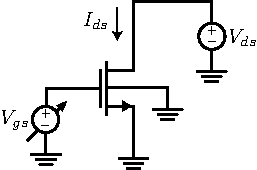
\includegraphics[width=.35\columnwidth]{idvgs_sweep} &
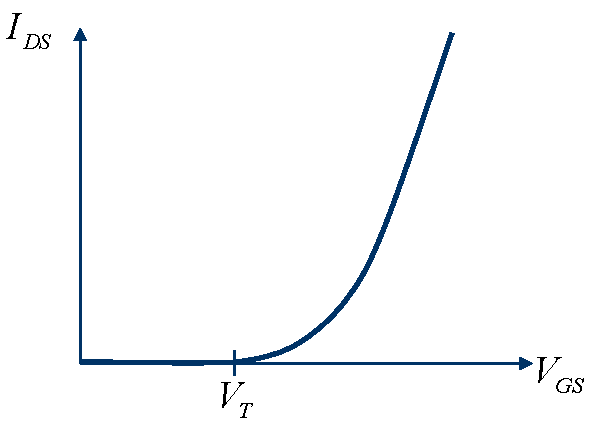
\includegraphics[width=.55\columnwidth]{mos_ids_vgs}\\
(a) & (b)\\
\end{tabular}
\caption{The $I_{DS}$ versus $V_{GS}$ characteristics of a MOSFET can be traced out by holding the drain voltage constant and sweeping the gate voltage as shown.}
\label{fig:idvgs_sweep}
\end{figure}
%%%%%%%%%%%%%%%%%%%%%%%%%%%%%%%%%%%%%%%%%%%%
As shown in Fig.~\ref{fig:idvgs_sweep}, suppose we connect an NMOS device gate to a voltage swept source and the drain to a positive voltage $V_{DS} > 0$V.  In this experiment, we monitor the drain-to-source current $I_{DS}$.  As shown, the current is initially zero and the transistor only conducts when the gate-to-source voltage exceeds a threshold.  As shown, the body of the transistor and source are both tied to ground, so in this case the gate-to-source voltage is also the gate-to-body voltage.  We know that when we cross the $V_T$ of the device, an inversion layer forms and this must be responsible for the current flow.
%%%%%%%%%%%%%%%%%%%%%%%%%%%%%%%%%%%%%%%%%%%%
We find that the current increases rapidly as we cross the threshold and it reaches a point where it simply increases linearly with applied gate-to-source voltage.  Also, if we zoom in to the region near the threshold, we'll observe very small conduction, in a region called "sub-threshold region", where minute current flow is possible.  We'll explain this current flow when we study bipolar junction transistors (BJTs), and in this chapter we'll ignore this region.  
%%%%%%%%%%%%%%%%%%%%%%%%%%%%%%%%%%%%%%%%%%%%
%             SUBSECTION 8.3.4             %
%%%%%%%%%%%%%%%%%%%%%%%%%%%%%%%%%%%%%%%%%%%%
\subsection{Observed Behavior: \texorpdfstring{$I_{DS} - V_{DS}$}{Drain Current vs. Drain Voltage}}
%%%%%%%%%%%%%%%%%%%%%%%%%%%%%%%%%%%%%%%%%%%%
%                 FIGURE                   %
%%%%%%%%%%%%%%%%%%%%%%%%%%%%%%%%%%%%%%%%%%%%
\begin{figure}[tb]
\centering
\begin{tabular}{cc}
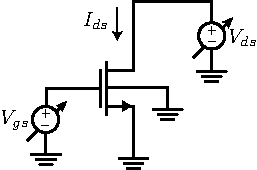
\includegraphics[width=.3\columnwidth]{idvds_sweep} &
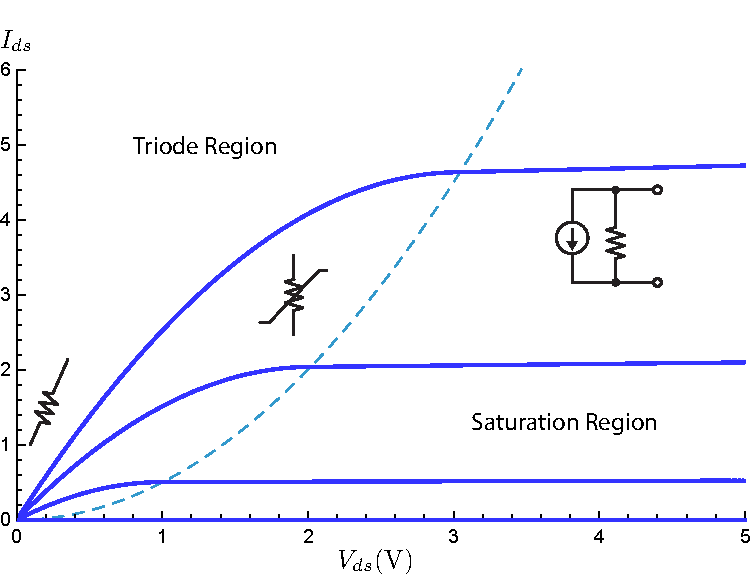
\includegraphics[width=.6\columnwidth]{ids_vds}\\
(a) & (b)\\
\end{tabular}
\caption{(a) The $I_{DS}$ versus $V_{DS}$ characteristics of a MOSFET can be traced out by holding the gate voltage constant and sweeping the drain voltage as shown.  (b) A family of curves results from varying the gate voltage in discrete steps.  Note that the device characteristics can be divided into two distinct regions.  In the "Triode Region" the device acts like a non-linear resistor whereas in the "Saturation Region" the current is relatively constant as a function of $V_{DS}$, acting like a current source.}
\label{fig:ids_vds}
\end{figure}
%%%%%%%%%%%%%%%%%%%%%%%%%%%%%%%%%%%%%%%%%%%%
Now suppose that we fix the gate voltage to constant values and sweep the drain-to-source voltage, as shown in Fig.~\ref{fig:ids_vds}.  What we observe is a family of curves, each curve corresponding to a particular value of the gate voltage.  Just as before, if the gate-to-source voltage is below the threshold, then no current flows and we observe the flat line at $0$A. For a gate-to-source voltage above threshold, we observe an $I$-$V$ behavior of a non-linear resistor.  For low values of drain-to-source voltage, the device is like a normal resistor. As the voltage is increased, the resistance behaves non-linearly and the rate of increase of current slows as the curve bends over.  
%%%%%%%%%%%%%%%%%%%%%%%%%%%%%%%%%%%%%%%%%%%%
Eventually the current stops growing and remains essentially constant, acting like a current source.  The dashed line separates the current into two regions, called the "Triode Region" and the "Saturation Region".  In the saturation region the current is saturated at a fixed value and increases very little for variations in the drain-source voltage.  We draw schematic symbols in each region to emphasize the behavior of the device, first as a conductor, then a non-linear conductor, and finally as a current source.
%%%%%%%%%%%%%%%%%%%%%%%%%%%%%%%%%%%%%%%%%%%%%%%%%%%%%%%%%%%%%%%%%%%%%%%%%%%%%%%%%%%%%%%%
%%%%%%%%%%%%%%%%%%%%%%%%%%%%%%%%%%%%%%%%%%%%%%%%%%%%%%%%%%%%%%%%%%%%%%%%%%%%%%%%%%%%%%%%
%                                   SECTION 8.4                                        %
%%%%%%%%%%%%%%%%%%%%%%%%%%%%%%%%%%%%%%%%%%%%%%%%%%%%%%%%%%%%%%%%%%%%%%%%%%%%%%%%%%%%%%%%
%%%%%%%%%%%%%%%%%%%%%%%%%%%%%%%%%%%%%%%%%%%%%%%%%%%%%%%%%%%%%%%%%%%%%%%%%%%%%%%%%%%%%%%%
\section{Derivation of MOSFET \texorpdfstring{$I-V$}{I-V} Curve}
With an understanding of the channel inversion forming due to the operating point of the MOS-C device, we can now derive the current flow due to the inversion layer.  Our derivations are approximate and simple to aid us in gaining insight into the device, not to build accurate models.
%%%%%%%%%%%%%%%%%%%%%%%%%%%%%%%%%%%%%%%%%%%%
%             SUBSECTION 8.4.1             %
%%%%%%%%%%%%%%%%%%%%%%%%%%%%%%%%%%%%%%%%%%%%
\subsection{MOSFET "Linear'' Region}
With reference to Fig.~\ref{fig:mos_triode}, let's assume the device is biased in inversion to allow current to flow:
    \begin{equation}
        {V_{GS}} > {V_{T}}
    \end{equation}
When the drain-to-source voltage is not too large, we observed that the device behaves like an ordinary conductor.  This makes sense if we view the channel as a semiconductor resistor.  Let's calculate the current to verify this.  
The current in this channel is given by
    \begin{equation}
        {I_{DS}} =  - W{v_y}{Q_N}
    \end{equation}
where $W$ is the width of the device, $v_y$ is the velocity of charge carriers in the $y$ direction (along the channel), and $Q_N$ is the inversion charge density at the surface.  
%%%%%%%%%%%%%%%%%%%%%%%%%%%%%%%%%%%%%%%%%%%%
The charge is proportional to the voltage applied across the oxide over threshold, or the \emph{overdrive voltage}.  "Overdrive" means a bias voltage applied over threshold.
    \begin{equation}
        {Q_N} = {C_{ox}}({V_{GS}} - {V_{T}})
    \end{equation}
Substituting this expression, we have
    \begin{equation}
        {I_{DS}} =  - W{v_y}{C_{ox}}({V_{GS}} - {V_{T}})
    \end{equation}
If we assume that the channel is of uniform density, only drift current flows.  The drift velocity of carriers is proportional to the electric field along the channel
    \begin{equation}
        {v_y} =  - {\mu _n}{E_y}
    \end{equation}
Notice that this electric field is different from the MOS-C vertical electric field, which is in the $x$ direction, with all field lines terminating on charges.  The lateral field is along the channel ($y$ direction), and for a uniform density of charges, is proportional to the drain-to-source voltage:
    \begin{equation}
        {E_y} =  - \frac{{{V_{DS}}}}{L}
    \end{equation}
where $L$ is the channel length, since this voltage is dropped uniformly across the channel.  Again, this assumption is only valid if the channel is uniform.  Making this last substitution completes the derivation of current versus voltage for the MOSFET in the linear regime:
    \begin{equation}
        {I_{DS}} = \frac{W}{L}{\mu _n}{C_{ox}}({V_{GS}} - {V_{Tn}}){V_{DS}}
    \end{equation}
Since current is proportional to voltage, we can define a channel conductance
    \begin{equation}
        G_{DS} = {{{\mu _n}{C_{ox}}({V_{GS}} - {V_{Tn}})}}\left( {\frac{W}{L}} \right)
    \end{equation}
This equation shows that the conductance depends on the carrier mobility $\mu_n$, the level of inversion $C_{ox}(V_{GS}-V_T)$, and the device dimensions. For a fixed aspect ratio $W/L$, we get more current by realizing higher mobility $\mu_n$, higher gate-oxide capacitance $C_{ox}$, and higher bias voltages.  
%%%%%%%%%%%%%%%%%%%%%%%%%%%%%%%%%%%%%%%%%%%%
%             SUBSECTION 8.4.2             %
%%%%%%%%%%%%%%%%%%%%%%%%%%%%%%%%%%%%%%%%%%%%
\subsection{MOSFET as a Variable Resistor}
Notice that in the linear region, the current is proportional to the drain-source voltage and the gate-source voltage.  For a fixed gate-source voltage, the equivalent resistance is given by $1/G_{DS}$.  We define a voltage-dependent resistor
    \begin{equation}
        {R_{eq}} = \frac{{{V_{DS}}}}{{{I_{DS}}}} = \frac{1}{{{\mu _n}{C_{ox}}({V_{GS}} - {V_T})}}\left( {\frac{L}{W}} \right) = {R_\Box}({V_{GS}})\frac{L}{W}
    \end{equation}
This is a variable resistor, electronically tunable by adjustment of the gate-to-source voltage.  The parameter $R_\Box$ is the sheet resistance of the surface of the MOS transistor, and the sheet resistance drops with increasing gate overdrive.
%%%%%%%%%%%%%%%%%%%%%%%%%%%%%%%%%%%%%%%%%%%%
%             SUBSECTION 8.4.3             %
%%%%%%%%%%%%%%%%%%%%%%%%%%%%%%%%%%%%%%%%%%%%
\subsection{Approximate Derivation of Inversion Charge Variation}
Up to now, we've ignored the fact that the level of inversion should vary from the source to the drain.  To understand why, consider that the channel covers the surface of the device and any gate voltage charge will be compensated by inversion charge in the channel.  If $V_{DS} \ne 0$V, then the channel potential is not uniform, and since the inversion charge depends on the gate-to-channel voltage, we should expect that the inversion charge to be maximum on the source side and lower on the drain side (because $V_{DS} > 0$V, as shown in Fig.~\ref{fig:mos_current_derive}).
%%%%%%%%%%%%%%%%%%%%%%%%%%%%%%%%%%%%%%%%%%%%
%                 FIGURE                   %
%%%%%%%%%%%%%%%%%%%%%%%%%%%%%%%%%%%%%%%%%%%%
\begin{figure}[tb]
\centering
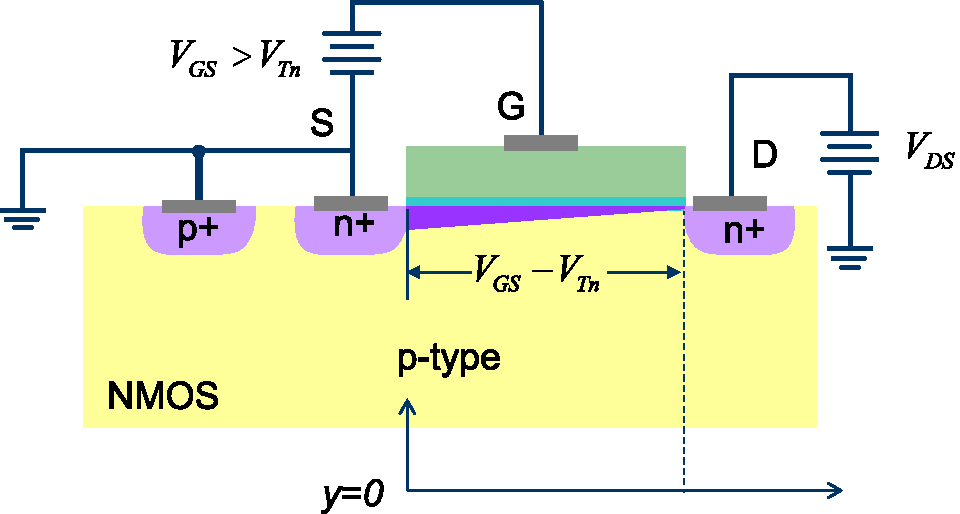
\includegraphics[width=.75\columnwidth]{mos_current_derive}
\caption{The setup to help derive the MOS current flow.  Note in particular the non-uniform inversion layer from the source side (maximum inversion) to the drain side (less inversion).}
\label{fig:mos_current_derive}
\end{figure}
%%%%%%%%%%%%%%%%%%%%%%%%%%%%%%%%%%%%%%%%%%%%
Let's approximate the  inversion charge $Q_N(y)$ along the channel, now a function of position along the channel $y$, by taking an average of the source/drain values:
    \begin{equation} 
        {Q_N}(y) \approx \frac{{Q_N}(y = 0) + {Q_N}(y = L)}{2} 
    \end{equation}
At the source side we have:
    \begin{equation} 
        {Q_N}(y = 0) =  - {C_{ox}}({V_{GS}} - {V_T}) 
    \end{equation}
while at the drain side we have
    \begin{equation} 
        {Q_N}(y = L) =  - {C_{ox}}({V_{GD}} - {V_T}) 
    \end{equation}
Note the gate-to-drain voltage is lower due to the higher potential at the drain side.  To see this, note that 
the voltage at the drain is given as the voltage at the source plus the $V_{DS}$
    \[
    	V_D = V_S + V_{DS}
    \]
    or
    \[
    	V_{GD} = V_{G} - V_{D} = V_{G} - (V_S + V_{DS}) = V_{GS} - V_{DS} 
    \]
resulting in less inversion charge at the drain side.  With this approximation, the average value of charge is given by
    \begin{equation}
        {Q_N}(y_{av}) \approx  - \frac{{{C_{ox}}({V_{GS}} - {V_T}) + {C_{ox}}({V_{GD}} - {V_T})}}{2}
    \end{equation}
Using this relation we have
    \begin{equation}
        {Q_N}(y) \approx  - \frac{{{C_{ox}}({V_{GS}} - {V_T}) + {C_{ox}}({V_{GS}} - {V_{DS}} - {V_T})}}{2}
    \end{equation}
Collecting terms, we have $2(V_{GS} - V_T)$ terms and one in terms of $V_{DS}$
    \begin{equation}
        {Q_N}(y) \approx  - \frac{{{C_{ox}}(2{V_{GS}} - 2{V_T}) - {C_{ox}}{V_{DS}}}}{2} =  - {C_{ox}}({V_{GS}} - {V_T} - \frac{{{V_{DS}}}}{2})
    \end{equation}
As expected, the average charge is lower than the source charge because the drain voltage is higher than the source, and so the vertical electric field is lower on the drain end, resulting in less inversion charge.
%%%%%%%%%%%%%%%%%%%%%%%%%%%%%%%%%%%%%%%%%%%%
%             SUBSECTION 8.4.4             %
%%%%%%%%%%%%%%%%%%%%%%%%%%%%%%%%%%%%%%%%%%%%
\subsection{Drift Velocity and Drain Current}
Now we use mobility to find velocity $v$ by approximating the $y$ direction field as before:
    \begin{equation}
        v(y) =  - {\mu _n}E(y) \approx  - {\mu _n}( - \Delta V/\Delta y) = \frac{{{\mu _n}{V_{DS}}}}{L}
    \end{equation}
This is clearly an approximation valid only under small $V_{DS}$.  Substituting into the expression for drift current, we have:
    \begin{equation}
        I_{DS} =  - Wv{Q_N} \approx W\mu \frac{{{V_{DS}}}}{L}{C_{ox}}({V_{GS}} - {V_T} - \frac{{{V_{DS}}}}{2})
    \end{equation}
Re-writing this into a form that emphasizes the geometric aspect ratio $W/L$:
    \begin{equation}
        I_{DS} = \frac{W}{L}\mu {C_{ox}}({V_{GS}} - {V_T} - \frac{{{V_{DS}}}}{2}){V_{DS}}
    \end{equation}
This leads to a family of inverted parabolas for the current as a function of $V_{DS}$.  These curves describe the channel conductance observed in Fig.~\ref{fig:ids_vds} wherein the current increases linearly but then bends as we increase $V_{DS}$.  We now understand the origin of the bend, since increasing $V_{DS}$ affects both the horizontal field along the channel (which tends to increase the current) but also results in lower levels of inversion in the channel, which tends to decrease the current.  These two effects essentially cancel out and the net result is a curve that is bending and flattening out.
%%%%%%%%%%%%%%%%%%%%%%%%%%%%%%%%%%%%%%%%%%%%
%             SUBSECTION 8.4.5             %
%%%%%%%%%%%%%%%%%%%%%%%%%%%%%%%%%%%%%%%%%%%%
\subsection{Square Law "Exact" Derivation}
It's hard to make claims of "exactness" because the actual equations are very complex.  We are still making many assumptions in the following derivation, but what follows will be less hand-wavy and a bit more precise.  The key insight is that the threshold voltage varies along the channel because the channel potential (call it $V_{ch}(y)$) is not constant from source to drain
    \begin{equation} 
        V_T(y) = V_T(y= 0 ) + V_{ch}(y) 
    \end{equation}
The threshold voltage at the drain end is related to the source end as follows:
    \begin{equation} 
        V_T(y=L) = V_T(y = 0) + V_D 
    \end{equation} 
since the higher drain potential requires a correspondingly higher gate voltage to reach the same level of inversion, exactly by the drain voltage.  That means the inversion charge varies from source to drain
    \begin{equation} 
        Q_n(y) = C_{ox} (V_G - V_T(y)) 
    \end{equation}
Or in other words, if we define $V_T$ as the threshold voltage at the source end ($V_T(y=0) = V_{T}$), the inversion charge varies as
    \begin{equation} 
        Q_n(y) = C_{ox} (V_G - V_T - V_{ch}(y) )  \label{eq:invcharge}
    \end{equation}
Using this, and the fact that the $E$-field is the spatial derivative of the channel voltage, we have
    \begin{equation} 
        I_{DS} = \mu_n W C_{ox} \left(V_G - V_T - V_{ch}(y) \right) \frac{dV_{ch}}{dy} 
    \end{equation}
Let's multiply both sides by $dy$ and integrate above along the channel.  We are converting the integral from position to voltage along the channel.  Since the current is uniform along the channel, the expression on the left-hand side must evaluate to $I_{DS} \times L$:
    \begin{equation} 
        \int_0^L I_{DS} dy = I_{DS} \cdot L = \int_0^{V_D} \mu_n W C_{ox} (V_G - V_T - V_{ch}(y)) dV_{ch} 
    \end{equation}
Resulting in the expression:
    \begin{equation} 
        I_{DS} = \mu_n C_{ox} \frac{W}{L} \left( V_G - V_T - \frac{V_D}{2} \right) V_D
        \label{eq:ids_triode}
    \end{equation}
Interestingly, this is the same equation we derived earlier.  While the result is that same, we have derived it in a way more consistent with the physics without resorting to hand-waving assumptions.  It should be noted that we have ignored one thing in this derivation, which is the variation of the threshold voltage due to the bulk depletion charges.  In \emph{Eq. ~\ref{eq:invcharge}}, we assume the inversion charge just varies linearly with the channel voltage. In practice, as the channel voltage increases from the source end, the depletion region width also changes, which means the threshold voltage is different. This is a subtle point that would over complicate the equations without providing more circuit insight or intuition, and it's common to make this simplification for hand calculations.
%%%%%%%%%%%%%%%%%%%%%%%%%%%%%%%%%%%%%%%%%%%%
The triode region current (\emph{Eq.~\ref{eq:ids_triode}}) is plotted in \emph{Fig.~\ref{fig:ids_triode_only}}.  We note that the currents peak when $V_{DS} = V_{GS} - V_T$, and then the equations predict lower and lower currents (inverted parabolas).  In the laboratory, we don't observe the current decreasing, and so there's a fundamental flaw in the derivation that we must address.  
%%%%%%%%%%%%%%%%%%%%%%%%%%%%%%%%%%%%%%%%%%%%
%                 FIGURE                   %
%%%%%%%%%%%%%%%%%%%%%%%%%%%%%%%%%%%%%%%%%%%%
\begin{figure}[tb]
\centering
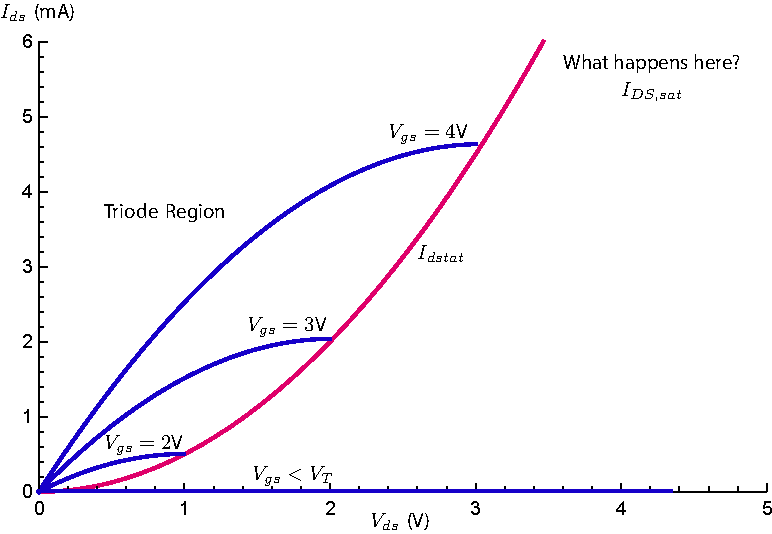
\includegraphics[width=.75\columnwidth]{ids_triode_only} 
\caption{The calculated family of MOSFET $I$-$V$ curves in the triode region.  The derivation here is only valid in the triode region and cannot predict the current saturation mechanism.}
\label{fig:ids_triode_only}
\end{figure}
%%%%%%%%%%%%%%%%%%%%%%%%%%%%%%%%%%%%%%%%%%%%%%%%%%%%%%%%%%%%%%%%%%%%%%%%%%%%%%%%%%%%%%%%
%%%%%%%%%%%%%%%%%%%%%%%%%%%%%%%%%%%%%%%%%%%%%%%%%%%%%%%%%%%%%%%%%%%%%%%%%%%%%%%%%%%%%%%%
%                                   SECTION 8.5                                        %
%%%%%%%%%%%%%%%%%%%%%%%%%%%%%%%%%%%%%%%%%%%%%%%%%%%%%%%%%%%%%%%%%%%%%%%%%%%%%%%%%%%%%%%%
%%%%%%%%%%%%%%%%%%%%%%%%%%%%%%%%%%%%%%%%%%%%%%%%%%%%%%%%%%%%%%%%%%%%%%%%%%%%%%%%%%%%%%%%
\section{Understanding Current Saturation (Pinch Off)}
%%%%%%%%%%%%%%%%%%%%%%%%%%%%%%%%%%%%%%%%%%%%
%                 FIGURE                   %
%%%%%%%%%%%%%%%%%%%%%%%%%%%%%%%%%%%%%%%%%%%%
\begin{figure}[tb]
\centering
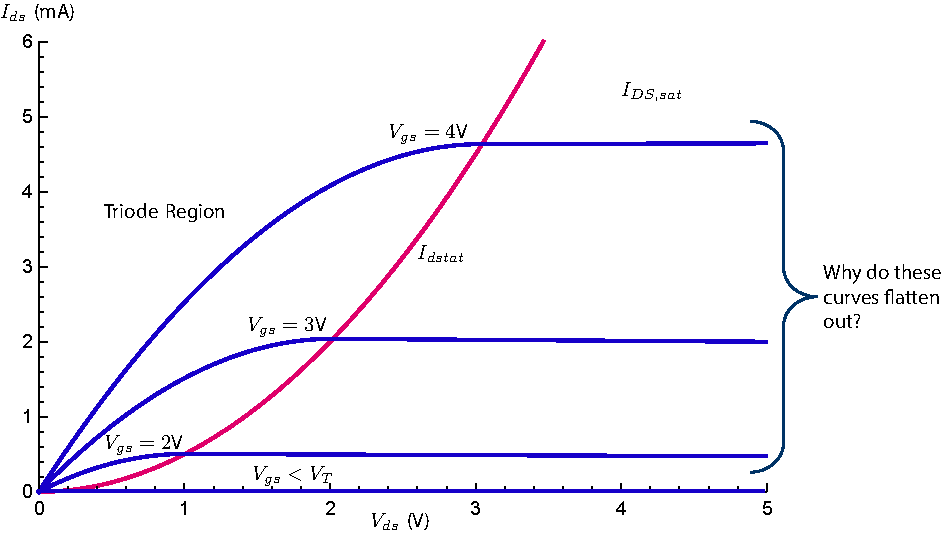
\includegraphics[width=.75\columnwidth]{ids_idsat_full} 
\caption{The piece-wise calculated MOSFET $I$-$V$ curves are derived by assuming the current in the saturation region is essentially constant and given by the maximum value predicted from the square-law relations.}
\label{fig:ids_family}
\end{figure}
%%%%%%%%%%%%%%%%%%%%%%%%%%%%%%%%%%%%%%%%%%%%
The observed experimental behavior of devices beyond a drain voltage of $V_{DS} = V_{GS} - V_T$ is a flattening of the current, rather than decreasing current.  Let's look into this a bit more to understand the origin of this saturation region, shown in Fig.~\ref{fig:mos_current_sat}.
%%%%%%%%%%%%%%%%%%%%%%%%%%%%%%%%%%%%%%%%%%%%
%             SUBSECTION 8.5.1             %
%%%%%%%%%%%%%%%%%%%%%%%%%%%%%%%%%%%%%%%%%%%%
\subsection{The Saturation Region}
From our equations, we have that when $V_{DS} > V_{GS} - V_T$, there is no inversion charge at the drain, so what happens? Intuitively it seems like the channel from the source to the drain is interrupted, or pinched off, so you might think this would lead to zero current again.  This intuition is so strong that this region is sometimes called the "pinch-off" region, but the current does not abruptly go to zero as intuition might lead you to believe.  
%%%%%%%%%%%%%%%%%%%%%%%%%%%%%%%%%%%%%%%%%%%%
%                 FIGURE                   %
%%%%%%%%%%%%%%%%%%%%%%%%%%%%%%%%%%%%%%%%%%%%
\begin{figure}[tb]
\centering
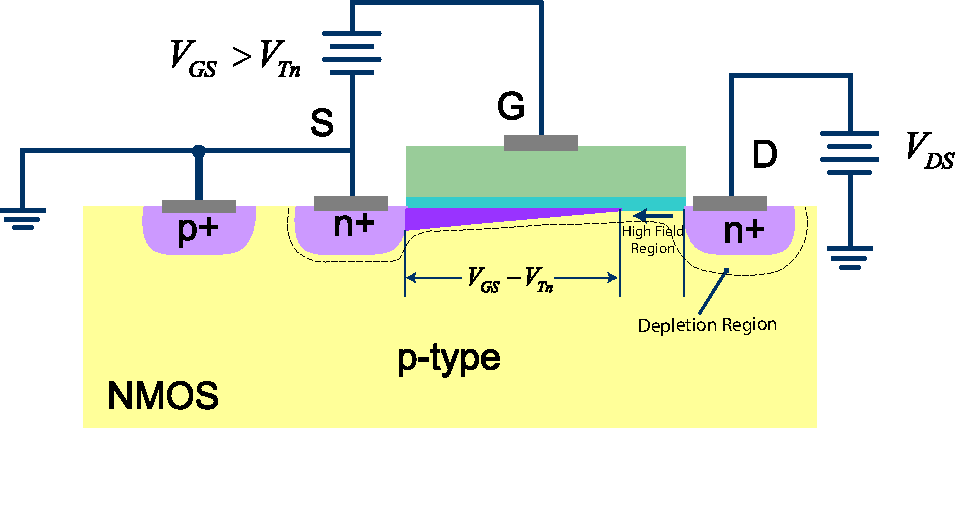
\includegraphics[width=.75\columnwidth]{mos_current_sat}
\caption{When a MOSFET is biased with $V_{DS} > V_{DS,sat}$, the channel is pinched off at a point inside but near the drain, creating a very small depletion region between the drain diffusion region and the conductive channel.  This region is a high $E$-field region.}
\label{fig:mos_current_sat}
\end{figure}
%%%%%%%%%%%%%%%%%%%%%%%%%%%%%%%%%%%%%%%%%%%%
%                 FIGURE                   %
%%%%%%%%%%%%%%%%%%%%%%%%%%%%%%%%%%%%%%%%%%%%
\begin{figure}[tb]
\centering
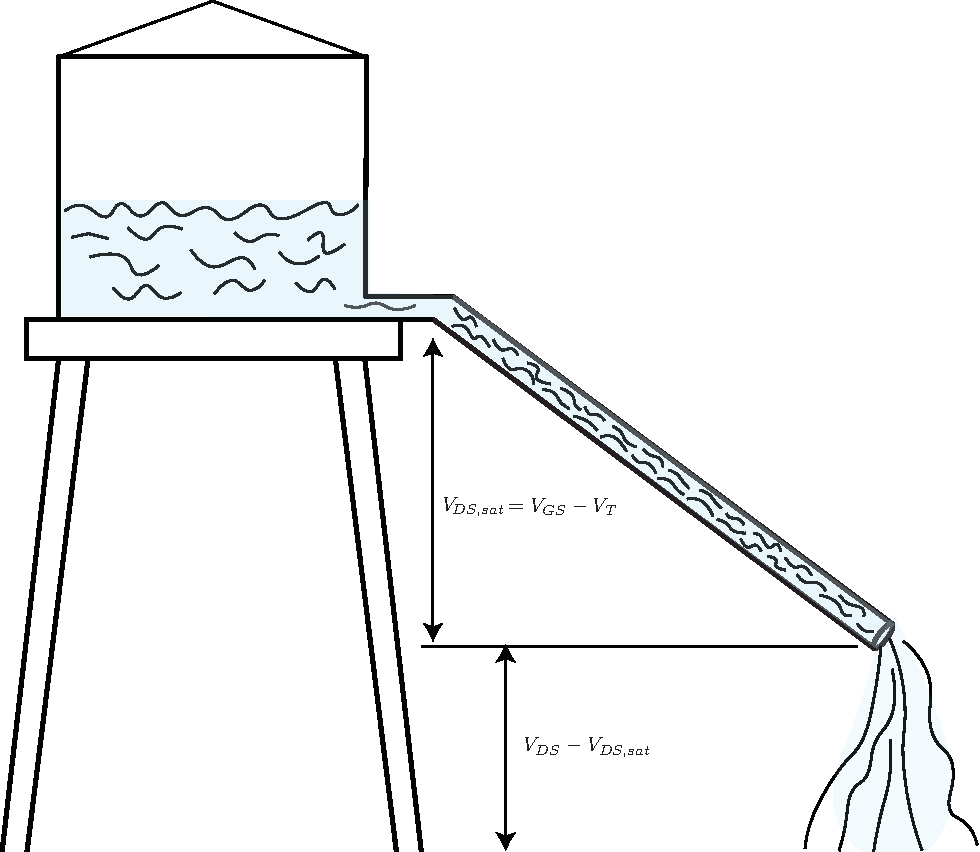
\includegraphics[width=.75\columnwidth]{waterfall}
\caption{A good analog for a MOSFET biased with $V_{DS} > V_{DS,sat}$ is a water pipe flowing down a hill into a waterfall.  The region where the water flows on the hill has a potential drop of $V_{DS,sat}$ and the remaining potential $V_{DS} - V_{DS,sat}$, is dropped through the waterfall.  The overall current is independent of the waterfall height.}
\label{fig:waterfall}
\end{figure}
%%%%%%%%%%%%%%%%%%%%%%%%%%%%%%%%%%%%%%%%%%%%
%             SUBSECTION 8.5.2             %
%%%%%%%%%%%%%%%%%%%%%%%%%%%%%%%%%%%%%%%%%%%%
\subsection{Pinch Off}
When $V_{DS} > V_{GS}-V_T$, we can say that the excess voltage $V_{DS} - (V_{GS}-V_T)$ is dropped across a small region between the drain and the channel, shown in Fig.~\ref{fig:mos_current_sat}.  Let's define $V_{DS,sat} = V_{GS}-V_T$ as the saturation drain voltage.  Any voltage above $V_{DS,sat}$ results in a fixed electric field $E_{d,sat}$ in the channel and an excess electric field $E_{d}$ near the drain end.  Since this is a small region, even a modest drain voltage above $V_{DS,sat}$ results in a potentially very large electric field $E_d$.  This large electric field can propel electrons from the channel into the drain end at high velocity.  In this region, increasing the drain voltage does not increase current (appreciably) because the current flow is limited by the supply of electrons from channel side, which is dictated by $E_{d,sat}$, set by $V_{DS,sat}$.  A good analogy is to imagine a stream of water gently flowing down an incline and then into a waterfall, as shown in Fig.~\ref{fig:waterfall}.  If the slope of the incline is increased, the current flow increases.  But the current flow is independent of the height of the waterfall.  In our system, the waterfall region is the high-field region.  
%%%%%%%%%%%%%%%%%%%%%%%%%%%%%%%%%%%%%%%%%%%%
In addition, in real transistors, current saturation may happen due to another mechanism, namely velocity saturation. If the field strength in the channel exceeds a threshold, the linear relation between drift velocity and electric field ceases to be valid and the velocity of carriers begins to saturate, as shown in Fig.~\ref{fig:ids_family}.
%%%%%%%%%%%%%%%%%%%%%%%%%%%%%%%%%%%%%%%%%%%%
%             SUBSECTION 8.5.3             %
%%%%%%%%%%%%%%%%%%%%%%%%%%%%%%%%%%%%%%%%%%%%
\subsection{Square-Law Current in Saturation}
Taking the above discussion into account, we can say that the current peaks at maximum value when 
$V_{DS} = V_{GS} - V_{T} = V_{DS,sat}$.  Or in other words:
    \begin{equation}
        I_{DS} = \frac{W}{L}\mu {C_{ox}}({V_{GS}} - {V_T} - \frac{{{V_{DS,sat}}}}{2}){V_{DS,sat}}
    \end{equation}
or 
    \begin{equation}
        {I_{DS,sat}} = \frac{W}{L}\mu {C_{ox}}({V_{GS}} - {V_T} - \frac{{{V_{GS}} - {V_T}}}{2})({V_{GS}} - {V_T})
    \end{equation}
This equation can be simplified into the following form:
    \begin{equation}
        {I_{DS,sat}} = \frac{W}{L}\frac{{\mu {C_{ox}}}}{2}{({V_{GS}} - {V_T})^2}
    \end{equation}
Notice that in the saturation region, the current is nearly independent of variations in the drain voltage and only depends on the gate voltage.  We can think of the transistor as an ideal voltage-controlled current source, with an output current dictated by the control terminal, the gate.  This is the characteristics of an ideal amplifier.
%%%%%%%%%%%%%%%%%%%%%%%%%%%%%%%%%%%%%%%%%%%%
%             SUBSECTION 8.5.4             %
%%%%%%%%%%%%%%%%%%%%%%%%%%%%%%%%%%%%%%%%%%%%
\subsection{Actual Saturation Current}
Now we need to do deal with another fact.  The measured values of  $I_{DS}$ increases slightly with increasing $V_{DS}$, in other words the curves are not 100\% flat.   The physics is complicated, but a simple way to see this is that the channel is getting shorter as the drain voltage depletes away more electrons from the drain end, resulting in a shorter channel length.   We can model this with an additional linear term $\lambda$ that allows the current to increase slightly for larger and larger $V_{DS}$ values:
    \begin{equation}
        {I_{DS,sat}} = \frac{W}{L}\frac{{\mu {C_{ox}}}}{2}{({V_{GS}} - {V_T})^2}(1 + \lambda {V_{DS}})
    \end{equation}
%%%%%%%%%%%%%%%%%%%%%%%%%%%%%%%%%%%%%%%%%%%%
%             SUBSECTION 8.5.5             %
%%%%%%%%%%%%%%%%%%%%%%%%%%%%%%%%%%%%%%%%%%%%
\subsection{Channel Length Modulation} \label{sec:mos_clm}
To see why the current increases, let's go back to when $V_{DS} = V_{GS} - V_T = V_{DS,sat}$, at which point the channel pinches off near the drain. With further increase in $V_{DS}$, we see that the pinch-off point moves toward the source, effectively reducing the channel length from $L$ to $L-\Delta L$, as shown in Fig.~\ref{fig:mos_current_sat_clm}.  Since current is inversely proportional to $L$, we have
    \begin{equation} 
        I_{DS} = \frac{1}{2}{\mu _n}{C_{ox}}\frac{W}{{L - \Delta L}}{\left( {{V_{GS}} - {V_T}} \right)^2} 
    \end{equation}
If $\Delta L \ll L$, we can simplify this to 
    \begin{equation} 
        I_{DS} = \frac{1}{2}{\mu _n}{C_{ox}}\frac{W}{L}{\left( {{V_{GS}} - {V_T}} \right)^2}  \left(1 - \frac{\Delta L(V_{DS})}{L} \right)
    \end{equation}
The change is $L$ as a function of $V_{DS}$ is known as Channel Length Modulation (CLM).  To first order
    \begin{equation} 
        \frac{\Delta L(V_{DS})}{L} = \lambda V_{DS}
    \end{equation}
Allowing us to write
    \begin{equation} 
        I_{DS} = \frac{1}{2}{\mu _n}{C_{ox}}\frac{W}{L}{\left( {{V_{GS}} - {V_T}} \right)^2}\left( {1 + \lambda {V_{DS}}} \right) 
    \end{equation}
Note that the channel length modulation parameter $\lambda$ has units of inverse volts, $\mathrm{V^{-1}}$.  Sometimes this parameter is called the "Early Voltage" 
    \begin{equation} 
        V_A = \frac{1}{\lambda}
    \end{equation}
The name "Early" is related to the Early Effect, named after its discoverer James M. Early, first applied to bipolar junction transistors.  
%%%%%%%%%%%%%%%%%%%%%%%%%%%%%%%%%%%%%%%%%%%%
%                 FIGURE                   %
%%%%%%%%%%%%%%%%%%%%%%%%%%%%%%%%%%%%%%%%%%%%
\begin{figure}[tb]
\centering
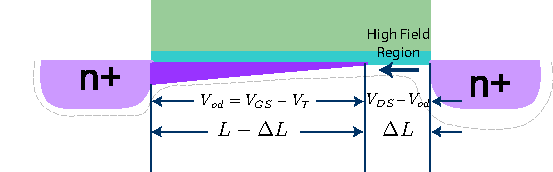
\includegraphics[width=.75\columnwidth]{mos_current_sat_clm}
\caption{Channel Length Modulation (CLM) occurs when the drain voltage is modulated beyond $V_{DS,sat}$.  The extra voltage dropped across the high-field region causes the effective channel length to shrink by $\Delta L$, which results in an increase in the drain-source current.}
\label{fig:mos_current_sat_clm}
\end{figure}
%%%%%%%%%%%%%%%%%%%%%%%%%%%%%%%%%%%%%%%%%%%%
%             SUBSECTION 8.5.6             %
%%%%%%%%%%%%%%%%%%%%%%%%%%%%%%%%%%%%%%%%%%%%
\subsection{Summary: Regions of Operation}
Let's now summarize the various regions of operation, beginning with cut-off, or $V_{GS} < V_T$:
    \begin{equation}
        I_{DS} = 0\mathrm{A}
    \end{equation}
Note: this is an approximation we will make in this class.  In later courses you will learn about sub-threshold conduction and leakage in the device.  
%%%%%%%%%%%%%%%%%%%%%%%%%%%%%%%%%%%%%%%%%%%%
Next, let's consider the "Linear Region", when the device acts like a variable conductor.  In this region  $V_{GS} > V_T$, but $V_{DS} \ll V_{GS} - V_T$, resulting in
    \begin{equation}
        {I_{DS}} = \frac{W}{L}{\mu _n}{C_{ox}}({V_{GS}} - {V_T}){V_{DS}}
    \end{equation}
In the "Triode Region", defined when the channel is inverted so $V_{GS} > V_T$, a drain voltage is applied to allow current to flow, but the drain voltage does not exceed the gate-overdrive voltage, $V_{DS} < V_{GS} - V_T = V_{DS,sat}$.  The current is governed by
    \begin{equation}
        {I_{DS}} = \frac{W}{L}{\mu _n}{C_{ox}}({V_{GS}} - {V_T} - \frac{{{V_{DS}}}}{2}){V_{DS}}
    \end{equation}
Finally, if the channel is inverted at the source side but not at the drain side, we are in the "Saturation Region".  In this region, $V_{GS} > V_T$, and $V_{DS} > V_{GS} - V_T = V_{DS,sat}$.  The current is nearly constant
    \begin{equation}
        {I_{DS,sat}} = \frac{W}{L}\frac{{\mu {C_{ox}}}}{2}{({V_{GS}} - {V_T})^2}(1 + \lambda {V_{DS}})
    \end{equation}
And only varies minutely due to the channel length modulation effect described earlier. 
%%%%%%%%%%%%%%%%%%%%%%%%%%%%%%%%%%%%%%%%%%%%%%%%%%%%%%%%%%%%%%%%%%%%%%%%%%%%%%%%%%%%%%%%
%%%%%%%%%%%%%%%%%%%%%%%%%%%%%%%%%%%%%%%%%%%%%%%%%%%%%%%%%%%%%%%%%%%%%%%%%%%%%%%%%%%%%%%%
%                                   SECTION 8.6                                        %
%%%%%%%%%%%%%%%%%%%%%%%%%%%%%%%%%%%%%%%%%%%%%%%%%%%%%%%%%%%%%%%%%%%%%%%%%%%%%%%%%%%%%%%%
%%%%%%%%%%%%%%%%%%%%%%%%%%%%%%%%%%%%%%%%%%%%%%%%%%%%%%%%%%%%%%%%%%%%%%%%%%%%%%%%%%%%%%%%
\section{The Complementary PMOS Device}
%%%%%%%%%%%%%%%%%%%%%%%%%%%%%%%%%%%%%%%%%%%%
%             SUBSECTION 8.6.1             %
%%%%%%%%%%%%%%%%%%%%%%%%%%%%%%%%%%%%%%%%%%%%
\subsection{PMOS Device}
So far, we have derived all of our equations for an NMOS device.  The  PMOS devices work exactly the same way, but with an $N$-type body and a channel made of positive charges (holes).  As noted earlier, the schematic symbol is also different, with an arrow corresponding to the direction of current flow from the source to the drain.  Notice that holes do flow from the source to drain, so unlike an NMOS device, here the arrow and the flow of carriers is the same.  The complete square law relation is shown in Fig.~\ref{fig:idspmos}.  Compared to the NMOS device, everything is upside down. This is only if we insist on keeping the same polarity for voltages and currents.  Let's define the current as $I_{SD}$, not $I_{DS}$.   Also $V_{SG}$ and $V_{SD}$ are positive for forward active regions, so in terms of these variables, the curves look right-side-up as shown in Fig.~\ref{fig:ids_pmos_negative}.
%%%%%%%%%%%%%%%%%%%%%%%%%%%%%%%%%%%%%%%%%%%%
%                 FIGURE                   %
%%%%%%%%%%%%%%%%%%%%%%%%%%%%%%%%%%%%%%%%%%%%
\begin{figure}[tb]
\centering
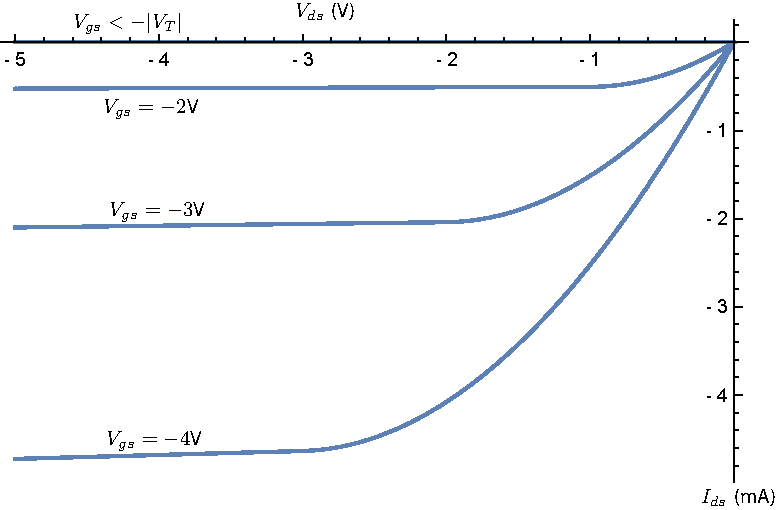
\includegraphics[width=.75\columnwidth]{idspmos}
\caption{PMOS $I$-$V$ curves are inverted compared to the NMOS curves because the current flows in the opposite direction (holes versus electrons), and the device is biased with a negative gate-to-source voltage in order to form the hole inversion channel.}
\label{fig:idspmos}
\end{figure}
%%%%%%%%%%%%%%%%%%%%%%%%%%%%%%%%%%%%%%%%%%%%
To derive the $I$-$V$ relation of a PMOS device without repeating all the steps above, we can simply invert all voltages and currents and arrive at the same equations.  For example, the saturation current is given by
    \begin{equation}
        {I_{SD,sat}} = \frac{W}{L}\frac{{\mu {C_{ox}}}}{2}{({V_{SG}} - {|V_{Tp}|})^2}(1 + \lambda {V_{SD}})
    \end{equation}
Since we inverted all the terms, we take an absolute value of the threshold voltage to make the equations identical with the NMOS case.  
%%%%%%%%%%%%%%%%%%%%%%%%%%%%%%%%%%%%%%%%%%%%
%                 FIGURE                   %
%%%%%%%%%%%%%%%%%%%%%%%%%%%%%%%%%%%%%%%%%%%%
\begin{figure}[tb]
\centering
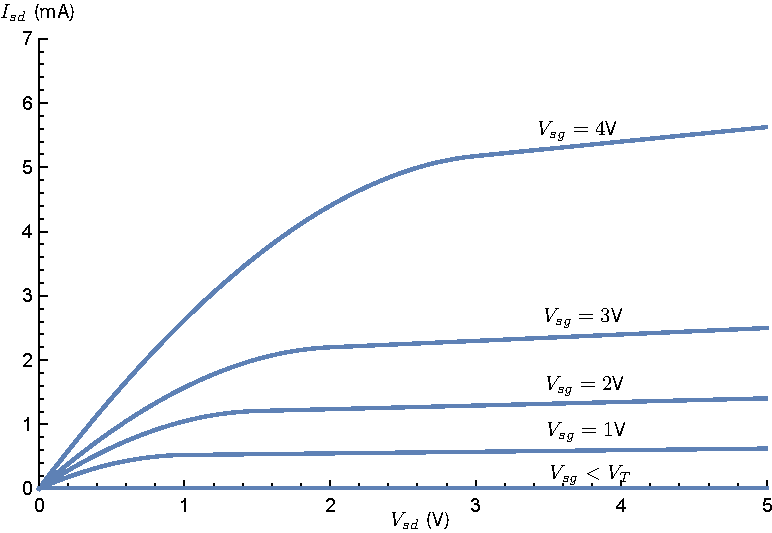
\includegraphics[width=.75\columnwidth]{ids_pmos_negative}
\caption{PMOS $I$-$V$ curves "right-side-up" by flipping the orientation of the device voltage and currents.}
\label{fig:ids_pmos_negative}
\end{figure}
